Habiendo definido nuestros algoritmos, lo que nos queda es ver cuál es la ventaja que otorgan los mismos en comparación a la solución naive de cada uno de estos problemas. Esta ventaja puede ser en precisión, tiempo o espacio. 

Para los experimentos utilizamos dos redes bayesianas, $\cancerNetwork$ y $\childNetwork$, tomadas del paquete de R \href{https://www.bnlearn.com/bnrepository/}{bnlearn}, podemos ver su estructura en la Figura \ref{fig:bayesian_networks_combined}. Utilizamos estas redes, ya que tenían un tamaño manejable y una topología similar a la de un polytree. Además de ser la distribución de nuestros datos, las empleamos como nuestros grafos causales, asumiendo que fueron generadas basándose en la causalidad \footnote{Esto no necesariamente siempre se cumple, pero entendemos que es una suposición razonable para la mayoría de los casos.}.
En el caso de la red \childNetwork, al no ser un polytree tuvimos que remover algunas aristas para lograr obtener esa estructura. Analizamos distintas heurísticas para remover ejes de la red convirtiéndola en un polytree. Utilizamos la más sencilla, que consiste en remover los ejes que generan ciclos en el grafo subyacente de la red bayesiana. Una opción más refinada consiste en elegir las aristas a remover, en base a cuáles minimizan la divergencia entre las distribuciones marginalizadas. Esto lo podríamos hacer comparando las distintas distribuciones que nos quedan al remover distintas aristas, utilizando una métrica como la divergencia de Kullback-Leibler, pero no era el objetivo de esta tesis. 

Para generar los datasets de entrenamiento y test, sampleamos instancias de ambas redes. Luego entrenamos al DT usando este dataset. A la hora de calcular el ASV, removimos la variable a predecir de nuestra red. Removemos la variable, puesto que si tuviéramos la red bayesiana completa con nuestra variable a predecir en la misma, haríamos la inferencia directamente en la red bayesiana \footnote{Tampoco entrenaríamos un árbol de decisión, sino que simplemente utilizaríamos a la red para clasificar las instancias}. Las variables que definimos para predecir fueron \variableNetwork{Smoker} y \variableNetwork{Age} para sus respectivas redes. En el caso de la red $\cancerNetwork$ no elegimos \variableNetwork{Cancer}, puesto que nuestro DAG causal iba a perder todas sus dependencias, por lo cual ASV no iba a poder detectar relaciones significativas. Luego en el caso de \childNetwork{} el criterio fue no utilizar una variable que se encuentre muy arriba en el árbol, puesto que no iba a tener muchas variables que la influencien, ni tan abajo que cueste distinguir las variables que la impactan mayormente. Por lo que nuestro input va a ser una red bayesiana $\aBayesianNetwork$, un feature a predecir $p$, un dataset $data$, un árbol de decisión $DT$ y una instancia $x \in data$. 

\begin{figure}[ht]
	\centering
	
	\begin{subfigure}[b]{0.3\textwidth}
		\centering
		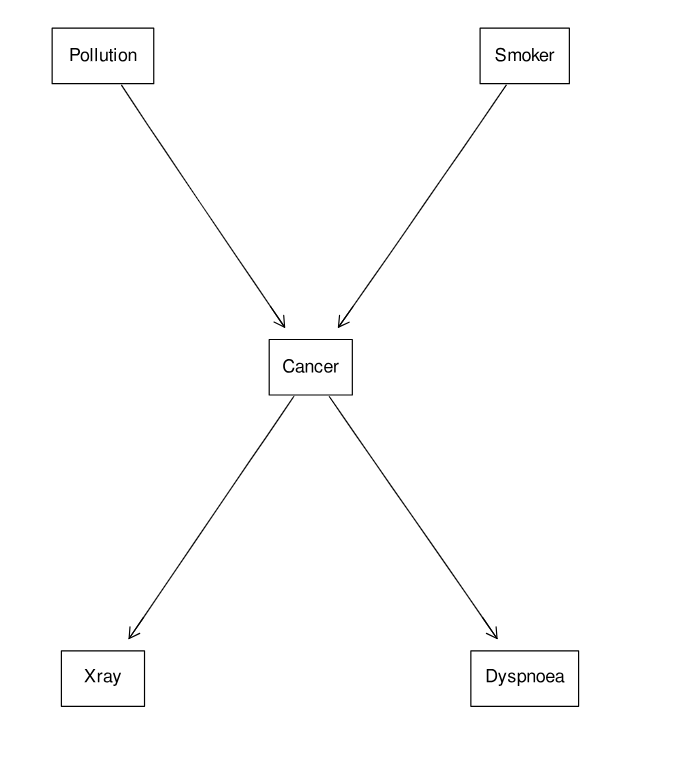
\includegraphics[width=\textwidth]{img/bayesianNetworks/cancerNetwork.png}
		\caption{Red Bayesiana $\childNetwork$ para analizar las enfermedades de niños de recién nacidos. Fuente: \cite{cancerNetwork}}
		\label{fig:cancer_network}
	\end{subfigure}
	\hfill
	\begin{subfigure}[b]{0.6\textwidth}
		\centering
		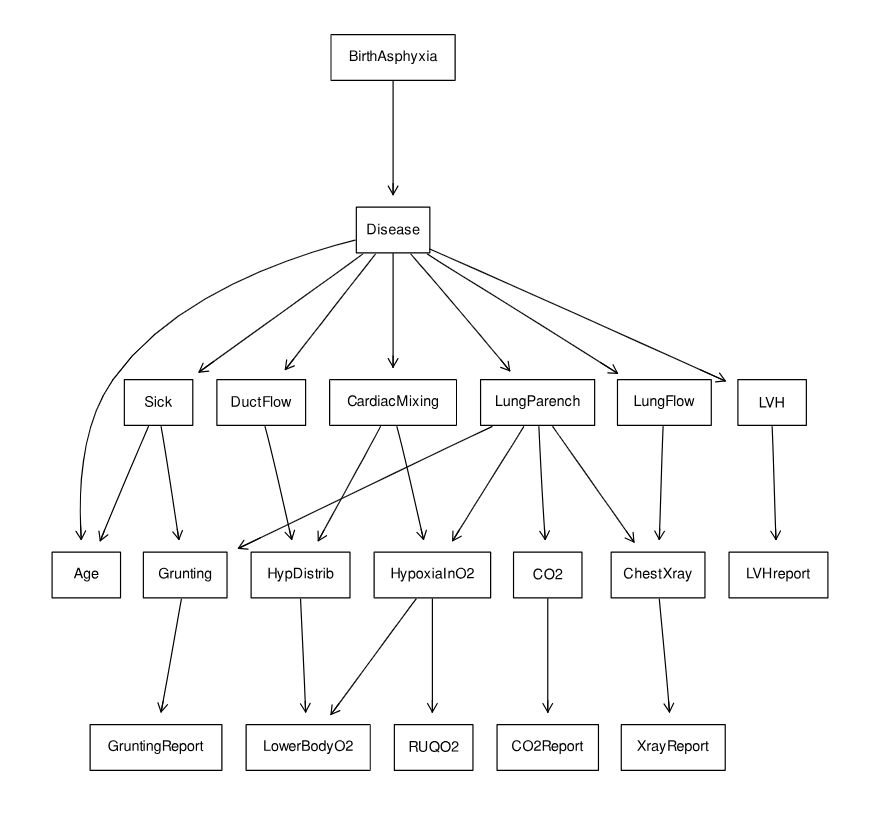
\includegraphics[width=\textwidth]{img/bayesianNetworks/childNetwork.png}
		\caption{Red Bayesiana \cancerNetwork para determinar la probabilidad de tener cáncer de distintos pacientes. Fuente: \cite{childNetwork}}
		\label{fig:child_network}
	\end{subfigure}
	
	\caption{Ejemplos de redes bayesianas utilizadas en los experimentos.}
	\label{fig:bayesian_networks_combined}
\end{figure}

\paragraph{Especificaciones de los experimentos}

\begin{itemize}
	\item \textbf{Procesador:} Intel(R) Core(TM) i5-7500 CPU @ 3.40GHz
	\item \textbf{Memoria RAM:} 16 GB
	\item \textbf{Sistema operativo:} Ubuntu 22.04 LTS
	\item \textbf{Python:} Versión 3.12
	\item  \textbf{Paquetes:} pgmpy (inferencia bayesiana), sklearn, networkx, shap
\end{itemize}

\subsection{Clases de equivalencia vs Órdenes Topológicos}

Para este experimento, vamos a comparar la implementación clásica de $ASV$ con nuestra idea de utilizar las clases de equivalencia para reducir los términos de la sumatoria. Para eso vamos a comparar la forma original de calcular ASV: 

$$\frac{1}{|topos(G)|} \sum_{\pi \in topos(G)} w(\pi) \left[ \charactheristicFunction(\pi_{<i} \cup {i}) - \charactheristicFunction(\pi_{<i}) \right] $$
con nuestra heurística:
$$\heuristicASVFormula$$

Hay dos métricas a tener en cuenta para ver cuál de estas dos estrategias es mejor. Primero, ver cuánto es el tiempo que se tarda en obtener los conjuntos sobre los que efectuar la sumatoria, que son $eqCl(G, x_i)$ y $topos(G)$. Luego comparar el tamaño de cada uno de esos conjuntos, puesto que por cada elemento de ese conjunto vamos a tener que evaluar a $\charactheristicFunction$ dos veces. Podría ocurrir que la construcción de las clases de equivalencia resulte computacionalmente costosa, y su cardinalidad no necesariamente presente una reducción significativa en comparación con $topos$. En tales casos, el costo adicional de calcularlas puede superar el beneficio esperado, incrementando el tiempo total de cómputo.

\begin{figure}[ht]
	\centering
	
\includegraphics[width=1\linewidth]{img/equivalentClassesVsToposorts.png}
	\caption[Caption for image]{Comparación de clases de equivalencias y órdenes topológicos de distintas clases de grafos. Se utiliza un promedio, puesto que la cantidad de clases de equivalencia depende del nodo que elijamos para calcularlas. \footnotemark }
	\label{fig:equivalenceClassesVsToposortsNumberPlot}
\end{figure}

\footnotetext{La función no es monótona, ya que no se utilizaron todos los grafos posibles para cada una de las clases mencionadas, se realizó una estimación a partir de una muestra significativa de distintos grafos de cada clase. }

%\echu{¿Es mejor tener un gráfico para cada familia? A mi me parecía mejor unificarlos} Queda unificado

Las distintas clases de grafos mencionados en la Figura \ref{fig:equivalenceClassesVsToposortsNumberPlot} son: 
\begin{itemize}
	\item Naive Bayes: Una red Naive Bayes con $n$ nodos, que tiene $n/2$ hojas y que tiene un camino de longitud $n/2-1$ en una de sus hojas. %\santi{No dan las cuentas de la cantidad de nodos} \echu{¿Ahí si, no? Me faltaba la raíz}
	\item Multiple paths: Un bosque compuesto de múltiples caminos de igual longitud. 
	\item Balanced tree: Un árbol binario perfecto balanceado.  
	\item Child network: La red bayesiana \childNetwork, sin algunos de sus ejes para ser un polytree. 
	
\end{itemize}

En la Figura \ref{fig:equivalenceClassesVsToposortsNumberPlot}, podemos observar como el número de clases de equivalencia crece significativamente más lento que el número de órdenes topológicos. Por ejemplo, en el caso de la red $\childNetwork$, la red tiene $7.41\times10^{11}$ órdenes topológicos y 2003 clases de equivalencia en promedio, por lo que si utilizamos las clases disminuimos enormemente la cantidad de llamadas a $\charactheristicFunction$. Luego, para los árboles balanceados, la cantidad de órdenes topológicos es $10^{50}$ veces mayor, una diferencia muy significativa. A partir de estos ejemplos, queda claro que es una mejora hacer el cálculo sobre las clases de equivalencia. Ahora solo queda ver el costo de calcularlas. 

El costo de calcular las clases lo podemos ver en la Figura \ref{fig:equivalenceClassesTimePlot}. Para la mayoría de los grafos de ejemplo que utilizamos tarda menos de 10 segundos. Pero para grafos de mayor tamaño, el tiempo que tarda comienza a crecer exponencialmente, al igual que la cantidad de clases de equivalencia. En el caso puntual de la red \childNetwork tarda menos de 1 segundo en calcular todas sus clases. 


\begin{figure}[ht]
	\centering
	
\includegraphics[width=1\linewidth]{img/equivalentClasses_time.png}
	\caption[Caption for image]{Comparación del tiempo en segundos que tarda el algoritmo para calcular las clases de equivalencia}
	\label{fig:equivalenceClassesTimePlot}
\end{figure}

\begin{figure}[ht]
	\centering
	
\includegraphics[width=1\linewidth]{img/equivalentClassesVsAllToposorts_time.png}
	\caption[Caption for image]{Comparación del tiempo en segundos que tarda el algoritmo para calcular las clases de equivalencia y calcular todos los órdenes topológicos, utilizando una \href{https://networkx.org/documentation/stable/reference/algorithms/generated/networkx.algorithms.dag.all_topological_sorts.html}{implementación} de la librería networkx. \footnotemark }
	\label{fig:equivalenceClassesVsToposortsTimePlot}
\end{figure}


\footnotetext{Para estimar el tiempo que tardaría se calcularon los primeros 1000 órdenes que devuelve el algoritmo exacto. Luego se utilizó ese tiempo para hacer una aproximación del tiempo total, sabiendo la cantidad de órdenes de cada grafo. Esto se realizó por simplicidad, ya que no era viable correr el algoritmo durante tanto tiempo.}

La Figura \ref{fig:equivalenceClassesVsToposortsTimePlot} nos muestra para distintos tipos de grafos cuánto tiempo toma cada algoritmo. En uno se obtienen todas las clases de equivalencia y en el otro todos los órdenes topológicos. A partir de $10^{15}$ órdenes topológicos el problema de calcularlos todos tardaría días, en cambio, calcular las clases de equivalencia sigue siendo una estrategia eficiente. Esto sucede así, puesto que, como vimos en el lema \ref{lemma:upper_bound_equivalence_classes}, la cantidad de clases de equivalencia depende de la estructura del grafo, y no de la cantidad de órdenes.
%\sergio{revisar esta frase, no tiene sentido que solo a partir de $10^{15}$ no es tratable} Rta: Ahí le puse la referencia al gráfico correspondiente y tuvo más sentido, si no era cualquier cosa. 

Por ende, a través de este experimento pudimos ver que la cantidad de clases de equivalencias es significativamente menor que la cantidad de órdenes, por lo que se reduce la cantidad de llamadas a $\charactheristicFunction$. Además, en la figura \ref{fig:equivalenceClassesVsToposortsTimePlot}, podemos ver cómo el tiempo para calcular las clases de equivalencia crece más lentamente que el tiempo de calcular todos los órdenes. Por lo tanto, podemos concluir que el algoritmo proporciona una mejora del tiempo para calcular todas las clases respecto a la implementación naive.
%\echu{Medio raro lo de doblemente efectiva, tal vez habría que expresarlo de otra forma}
%\sergio{Decir algo de que cambia el slope en la escala logarítmica notablemente}

\subsection{ASV exacto sin EqClasses vs ASV aproximado}

El objetivo de este experimento es comparar la performance de obtener los órdenes topológicos de un grafo que es un polytree, pero no es un \dtree. Por lo tanto, solo los podemos obtener sampleándolos con nuestro Algoritmo \ref{alg:topoSortSampling} o generándolos con el algoritmo de Knuth, puesto que las clases de equivalencia solo las podemos obtener para los \dtrees.

\begin{table}[h]
	\centering
	\begin{tabular}{|l|c|}
		\hline
		\textbf{Cantidad de órdenes sampleados} & \textbf{Tiempo de sampleo (s)}\\
		\hline
		100 & 0.9270 \\
		1000 & 1.1170 \\
		10000 & 4.7170 \\
		20000 & 7.7170 \\
		30000 & 10.8387 \\
		\hline
	\end{tabular}
	
	\caption{Tiempos de ejecución en segundos para muestreo y generación de órdenes topológicos de la red $\childNetwork$}
	\label{table:exactVsApproximateTopoSorts}
\end{table}

En la Tabla \ref{table:exactVsApproximateTopoSorts} podemos ver que el enfoque aproximado toma un tiempo tratable para samplear los órdenes. Aunque en nuestro análisis de la complejidad del mismo, habíamos llegado a una cota cuasi polinomial, el algoritmo se comporta de mejor manera en la práctica. También podemos observar que, como se mencionó al introducir el algoritmo de sampleo, su complejidad no es lineal en la cantidad de órdenes sampleados. Esto ocurre, pues vamos obteniendo múltiples candidatos en cada llamado recursivo de la función. 

En base a estos resultados, uno podría creer que la mejor opción es generarlos con el algoritmo de Knuth, el cual tarda menos de 1 segundo en generar los 30000 órdenes. El problema de este algoritmo es que no respeta la distribución de los órdenes.  Por ejemplo, si tuviéramos un grafo como el de la Figura \ref{fig:badExactToposortExample}, podría ocurrir que los primeros 1000 órdenes que nos devuelva el algoritmo tengan como primer nodo a $n_1$. Pero en realidad $n_1$ es el primer nodo en menos del 0.05\% de los casos, por ende no sería una muestra representativa. Para lograr esto deberíamos generar todos los órdenes, pero ya generar meramente un 1\% de los órdenes de la red $\childNetwork$ tomaría más de 2 días. 

%\echu{Este ejemplo, no tan detallado, lo mencionó también en el segundo parrafo de la sección de sampleo. ¿Vale la pena este experimento? Para mi esta bueno para ilustrar porque no garpa usar el algoritmo de Knuth, aunque no sume tantooo}

%\santi{Me parece bien.}

\begin{figure}[ht]
	\centering
	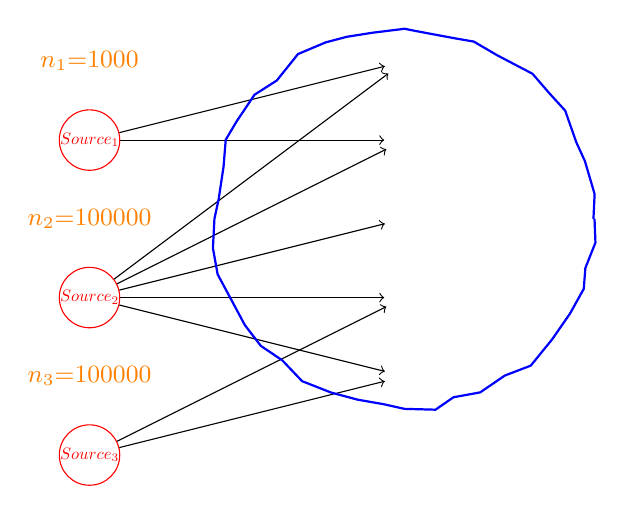
\begin{tikzpicture}
		% Define the rigth set of nodes
		\foreach \i in {1,2,3,4,5}
		\node[draw=none, circle, minimum size=5mm, inner sep=0pt] (L\i) at (4, -\i) {};
		
		% Define the left set of nodes
		\foreach \j in {1,2,3}
		\node[draw, circle, red, minimum size=5mm, inner sep=0pt] (source\j) at (0, -\j*2) {\scalebox{0.6}{$Source_\j$}};
		
		% Draw edges between nodes (example edges)
		\foreach \i in {1,2}
		\foreach \j in {1,2}
		\draw[->]  (source\j) -- (L\i); 
		
		\foreach \i in {4,5}
		\foreach \j in {2,3}
		\draw[->]  (source\j) -- (L\i); 
		
		\draw[->]  (source2) -- (L3);
		
		
		\draw [decorate, blue, decoration={random steps, segment length=10pt, amplitude=2pt}, thick]
		(4,-3) circle (2.4);
		
		%Número de ordenes topológicos para cada nodo
		
		\node[draw=none,minimum size=3mm, inner sep=0pt] () at (0, -1) {\small \textcolor{orange}{$n_1$=1000}};
		
		\node[draw=none,minimum size=3mm, inner sep=0pt] () at (0, -3) {\small \textcolor{orange}{$n_2$=100000}};
		
		\node[draw=none,minimum size=3mm, inner sep=0pt] () at (0, -5) {\small \textcolor{orange}{$n_3$=100000}};
	\end{tikzpicture}
	\caption{Posible comienzo del algoritmo exacto, con los candidatos a ser el primer nodo del orden en rojo y el resto del grafo en azul. Cada node fuente (source) tiene sus respectivas cantidades de órdenes topológicos en los que está primero.}
	\label{fig:badExactToposortExample}
\end{figure}

Por último, realizamos un experimento para calcular el error al calcular $ASV$ con el método aproximado, sampleando 1000 órdenes topológicos de la red $\childNetwork$. En la Figura \ref{fig:boxplotASVApproximateDifferences} podemos ver los resultados de esta corrida. La mayoría de los valores aproximados obtenidos tiene un error del 8\% con respecto a su valor exacto. Las diferencias más altas se corresponden a valores de $ASV$ muy pequeños, como 0.005, por lo que una pequeña diferencia en su valor calculado relativamente es más significativa. Esto es esperable, ya que el error mencionado en el Teorema \ref{theorem:asvSamplingError} es un error absoluto, no relativo. Para los features con valores mayores a 0.01, su diferencia es menor al 5\%.
%\santi{Esto es esperable: nuestro teorema habla de error absoluto, no del relativo. Podrías decirlo.}
Con estos resultados, podemos concluir que no es necesario obtener todos los ordenes y con una buena aproximación podemos obtener resultados medianamente precisos. 


\begin{figure}
	\centering
	
\includegraphics[width=0.8\linewidth]{img/asvResults/ChildAllSeedsASVBoxplot.png}
	\caption{Diferencia relativa entre los valores del ASV aproximado y el exacto para la red $\childNetwork$, se utilizaron las diferencias de 30 seeds. Estos son los valores mayores a 0.01.}
	\label{fig:boxplotASVApproximateDifferences}
\end{figure}
